\chapter{Concepts of Statistical Physics,
         Nearly Independent Particle Systems}

\section{微观状态的描写}

粒子,子系:院子,分子,振子,自旋,

	    ($\bm q$, $\bm p$), $q^a = 1$, $r$, $\epsilon(\bm q,\bm p)$

\[\d\omega = \d^r q \d^r p\]

$N$: $q_1$, ...,  $q_s$, $p_1$, ..., $p_s$. $s = Nr$

$\d\Omega = \d^s q \d^s p$ 

\[\Gamma = \{(q_1,...,q_s;p_1,...,p_s)\}\]
称为相空间.

$(q,p)$ 相空间中一个点,叫做一个微观状态.

量子:单粒子的量子态由一组守恒的量子数标志.

用一组可对易力学量算符的本征值描述.

例如,自由粒子:动量本征值

量子经典对应:单粒子量子态 <-> $\Delta \omega = h^r$ 的单粒子相阵积元.

全同性:

\section{等几率原理}

\begin{itemize}
  \item 对孤立系,$E$, $V$, $N$ 固定,最简单朴素的假设就是等几率假设:
  对于处于平衡态下的孤立系,系统各个可能的微观状态出现的几率相等.
  \item 可能的微观状态是指与宏观状态 $E$, $\nu$, $N$ 相容的经典或量子态.
\end{itemize}

\section{近独立粒子系统的统计物理}

\begin{itemize}
  \item 近独立是指相互作用很弱(只对体系达到平衡起作用)
  \begin{equation}
      E = \sum_{i=1}^N \epsilon_i
  \end{equation}
  \item $\epsilon_{n,\alpha}$, $\alpha = 1$, 能级指标. $g_\alpha$ 称为简并度.
  $a_\alpha$ 指每一个能级上的占有数.

  E.g.:
  \[
  \begin{tikzpicture}[baseline]
    \draw (0,0) node [left] {$\epsilon_1$} --++ (2,0);
    \draw (0,1) node [left] {$\epsilon_2$} --++ (2,0);
    \draw (0,2) node [left] {$\epsilon_3$} --++ (2,0);
  \end{tikzpicture}
  \Rightarrow
  \begin{tikzpicture}[baseline]
    \draw [dashed] (0,0) node [left] {$g_1 = 3$} --++ (2,0);
    \draw [dashed] (0,1) node [left] {$g_2 = 4$} --++ (2,0);
    \draw [dashed] (0,2) node [left] {$g_3 = 3$} --++ (2,0);
  \end{tikzpicture}
  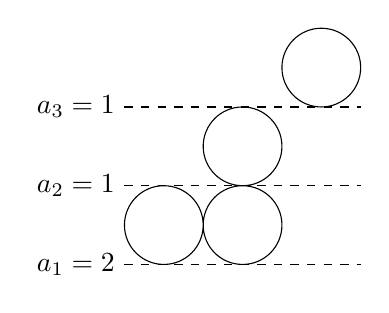
\begin{tikzpicture}[baseline]
    \draw [dashed] (0,0) node [left] {$a_1 = 2$} --++ (3,0);
    \draw [dashed] (0,1) node [left] {$a_2 = 1$} --++ (3,0);
    \draw [dashed] (0,2) node [left] {$a_3 = 1$} --++ (3,0);
    \draw (.5,.5) circle (.5) (1.5,.5) circle (.5) (1.5,1.5) circle (.5) (2.5,2.5) circle (.5);
  \end{tikzpicture}
  \]
  or another distribution
  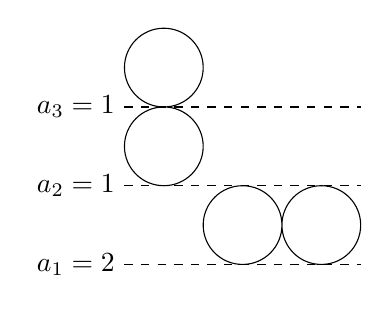
\begin{tikzpicture}[baseline]
    \draw [dashed] (0,0) node [left] {$a_1 = 2$} --++ (3,0);
    \draw [dashed] (0,1) node [left] {$a_2 = 1$} --++ (3,0);
    \draw [dashed] (0,2) node [left] {$a_3 = 1$} --++ (3,0);
    \draw (1.5,.5) circle (.5) (2.5,.5) circle (.5) (.5,1.5) circle (.5) (.5,2.5) circle (.5);
  \end{tikzpicture}

  能级 \quad 能极简并度
  \item  对孤立子
  \[\sum_\alpha a_\alpha = N, \sum_\alpha \epsilon_\alpha a_\alpha = E\]
  \item 对一个给定的 $\{a_\alpha\}$, 可以有不同的量子态. $\Rightarrow W(\{a_\alpha\})$
  等几率原理 $\{a_\alpha\}$ 出现的几率 $\propto$ $W\{a_\alpha\}$.
\end{itemize}

如果可区分 $W(\{a_\alpha\}) = \frac{N!}{\prod_\alpha a_\alpha!} \prod_\alpha g_\alpha^{a_\alpha}$,
Fermion $W_F(\{a_\alpha\}) = \prod_\alpha \frac{g_\alpha!}{a_\alpha!(g_\alpha - a_\alpha)!}$,
Boson $W_B(\{a_\alpha\}) = \prod_\alpha \frac{(g_\alpha + a_\alpha - 1)}{a_\alpha!(g_\alpha - 1)!}$.
